\chapter{Selection}
\begin{itemize}
	\item Naive samply vs. evolution 
	\item Notion of fitness 
	\item Dynamics of fitness distributions: 
	\begin{enumerate}
		\item Cumutants and GF 
		\item Asymptotic 
		\item Universality 
		\item Comparison with EVT
	\end{enumerate}
\end{itemize}

\section{Naive sampling}

$n$ components, each with probability $p$,

$$Prob(success)= p^n$$

For $p=\frac{1}{2}$ and $n=100$, $2^{-100}=8\cdot 10^{-31}$ ($1kg/mass$)
\begin{figure}[!h]
% Use "\centering" in floats (figure, table), but if you need to center
% some text (why?) use "\begin{center}...\end{center}".
\centering 
% Figure environments same as 0.8 * \textwidth please
% That does not necessarily mean the actual picture size,
% it is a guideline for the environment which could contain
% 2 or more pictures! Be consistent and follow the guidelines
% provided in your sources.
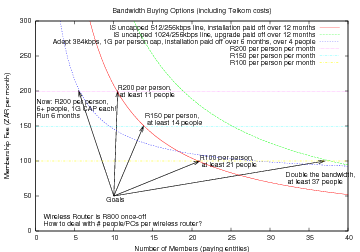
\includegraphics[width=0.8\textwidth]{images/bandwidth-colour.png}
\caption{Planning community bandwidth sharing costs. 
  Note caption capitalization.}
\label{bandwidth} 
% if you move the label it breaks the reference numbering; 
% always have it *after* the caption.
\end{figure}

Remember how to include code with {\tt verbatim} 
and to fix the tabs in {\sf python} in a verbatim environment? 
It may be best to have an `include' command for code, 
not to have to re-edit it all the time.
\verbatimtabinput{code/mycode.py}

\section{Selection: exponential amplification of rare events}

